\documentclass{standalone}
\usepackage{tikz}
\begin{document}
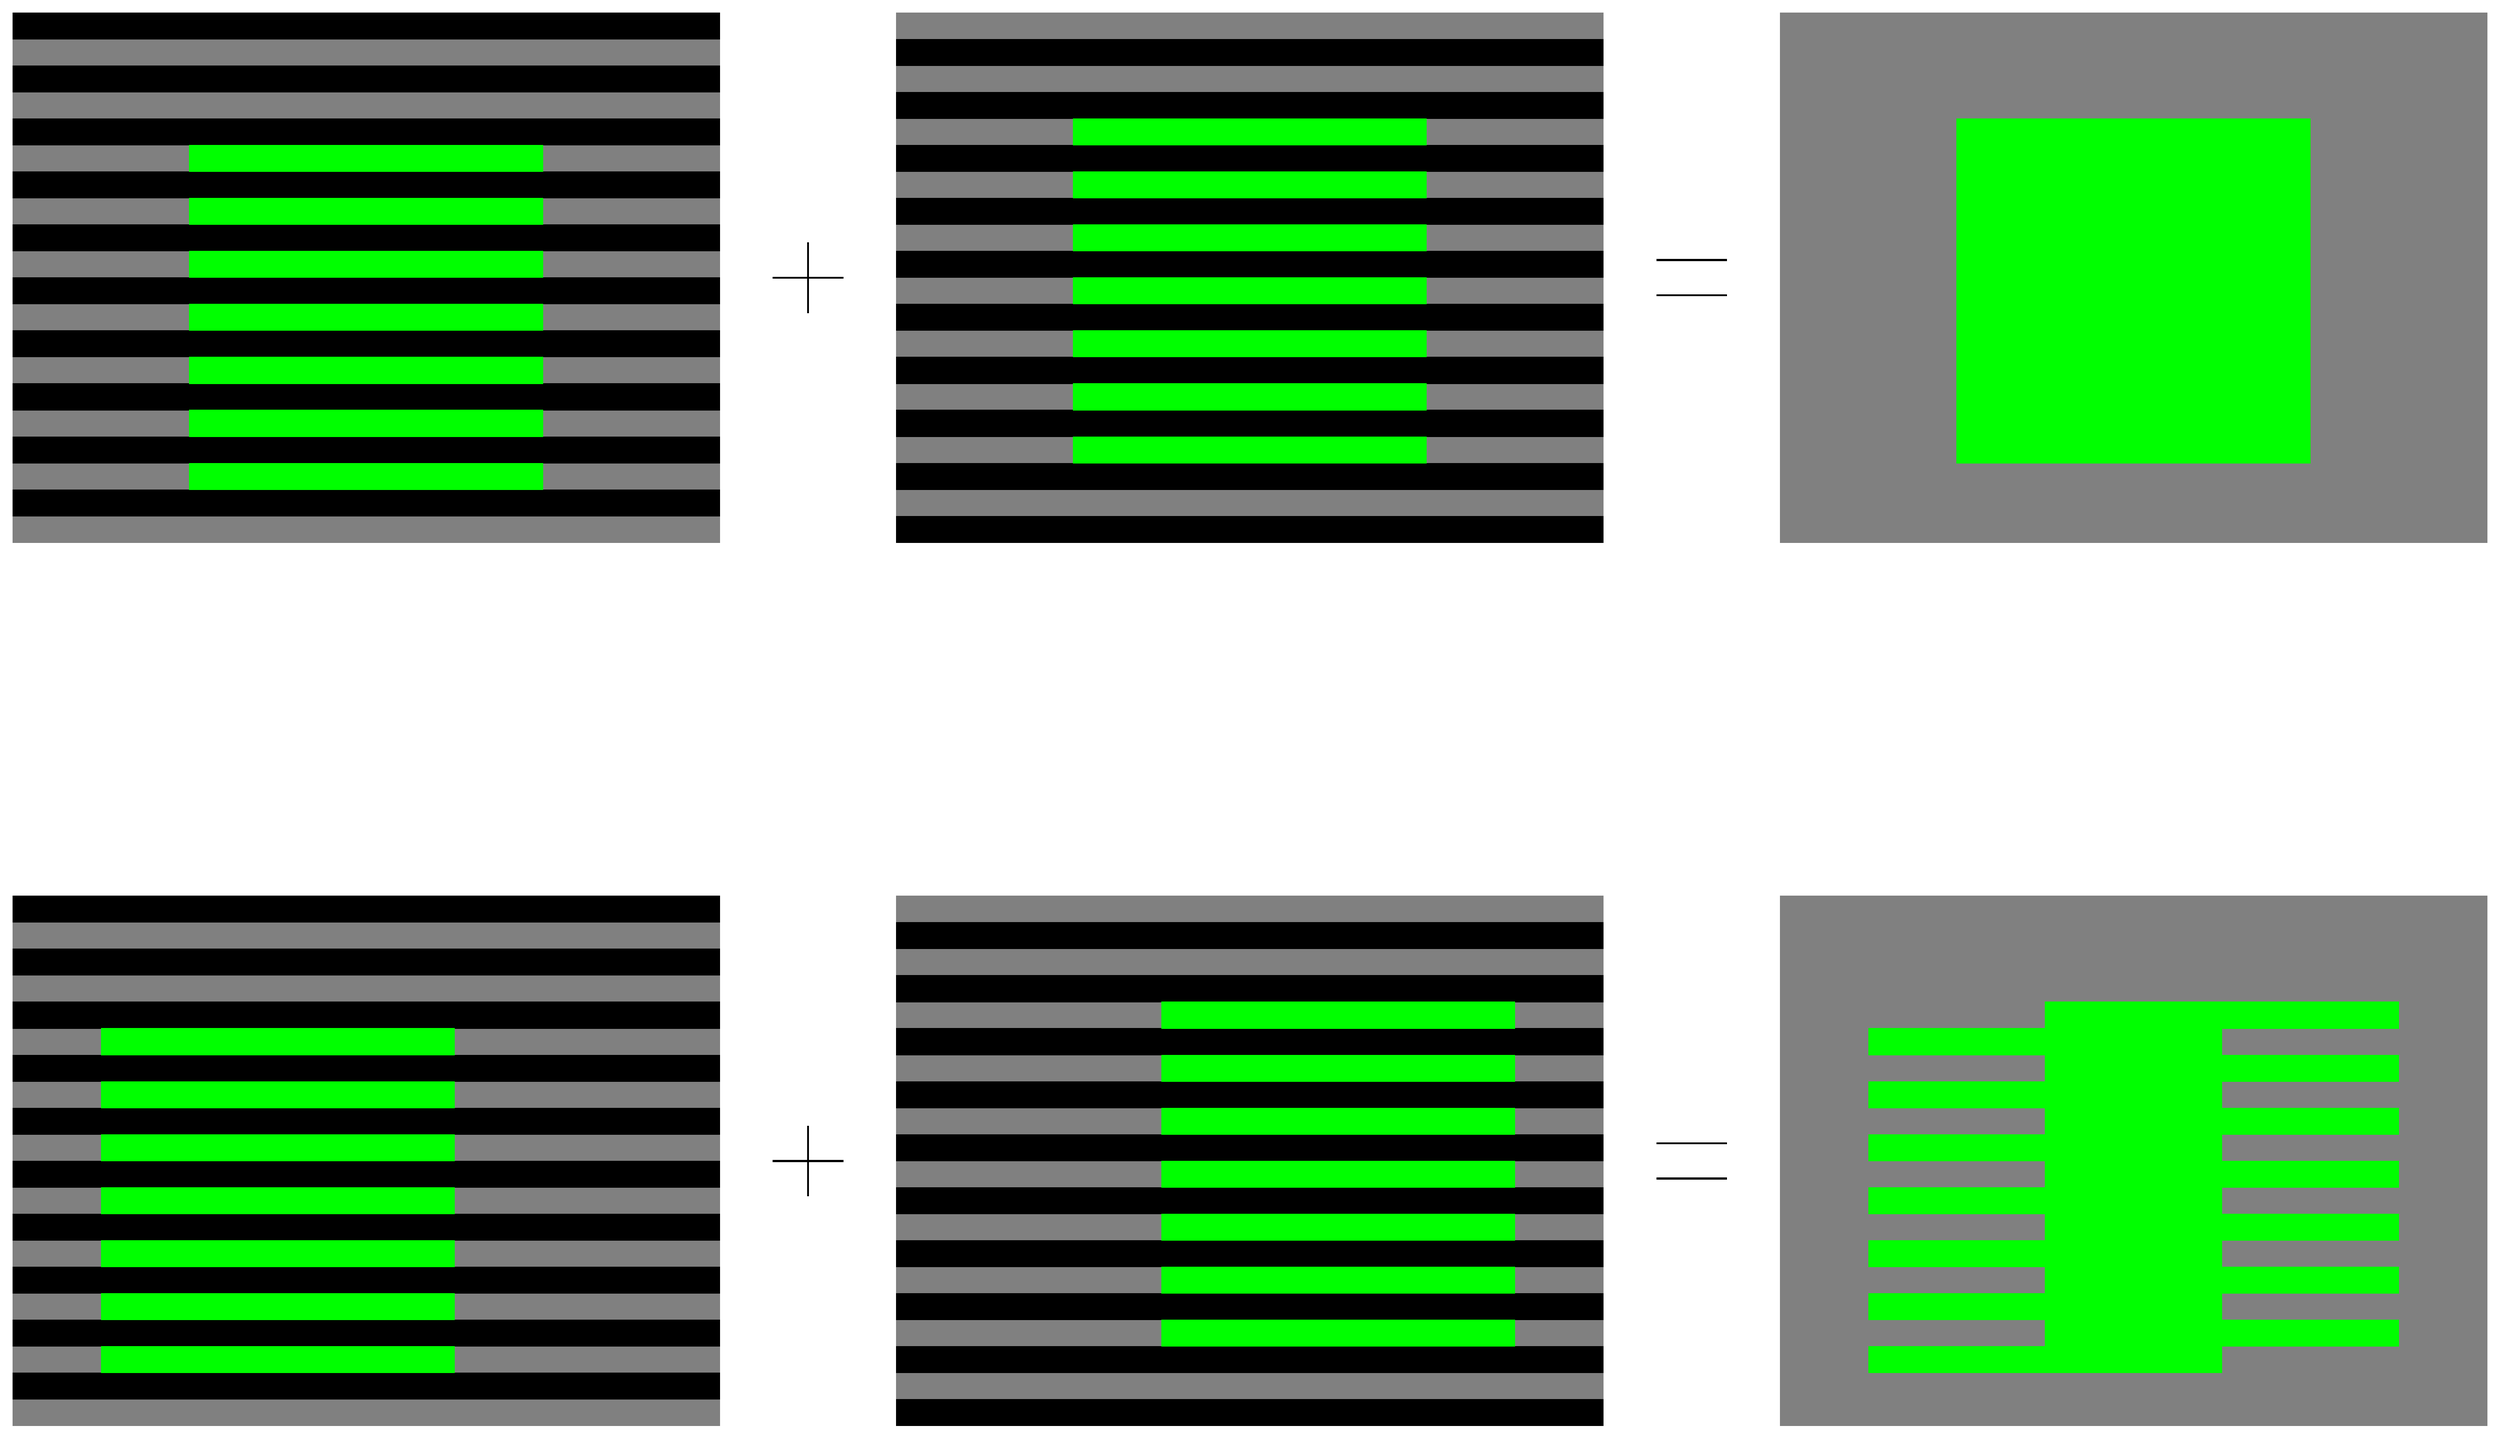
\begin{tikzpicture}[scale=5]

\def\wid{4.0}
\def\hei{3.0}
\def\objectsize{1.0}
\def\clrback{gray}
\def\clrobject{green}
\def\clrblank{black}
\def\numlines{20}
\def\lastline{19}

\def\firstvisible{3}
\def\lastvisible{15}

% \myboxes{middlex}{w}{firstindices}{color}
\newcommand*{\myboxes}[4]{
	\foreach \y in {#3}{
		\draw [#4,fill] (#1-0.5*#2,\y*\hei/\numlines) rectangle ++(#2,\hei/\numlines);
	}
}

	\myboxes{0}{\wid}{0,2,...,\lastline}{\clrback}
	\myboxes{0}{\wid}{1,3,...,\lastline}{\clrblank}
	\myboxes{0}{0.5*\wid}{2,4,...,\lastvisible}{\clrobject}

	\draw [ultra thick] (2.5, \hei/2) ++ (0.2, 0) -- ++(-0.4, 0) ++ (0.2, 0.2) -- ++(0, -0.4);
	% \node at (2.5, \hei/2) {\Huge +};

	\myboxes{5}{\wid}{1,3,...,\lastline}{\clrback}
	\myboxes{5}{\wid}{0,2,...,\lastline}{\clrblank}
	\myboxes{5}{0.5*\wid}{3,5,...,\lastvisible}{\clrobject}

	\draw [ultra thick] (7.5, \hei/2) ++(-0.2, 0.1) -- ++(0.4, 0) ++(0, -0.2) -- ++(-0.4, 0);
	%\node at (7.5, \hei/2) {\Huge =};

	\myboxes{10}{\wid}{0,1,...,\lastline}{\clrback}
	\myboxes{10}{0.5*\wid}{3,4,...,\lastvisible}{\clrobject}

\begin{scope}[yshift = -5cm]
	\myboxes{0}{\wid}{0,2,...,\lastline}{\clrback}
	\myboxes{0}{\wid}{1,3,...,\lastline}{\clrblank}
	\myboxes{-0.5}{0.5*\wid}{2,4,...,\lastvisible}{\clrobject}

	\draw [ultra thick] (2.5, \hei/2) ++ (0.2, 0) -- ++(-0.4, 0) ++ (0.2, 0.2) -- ++(0, -0.4);
	%\node at (2.5, \hei/2) {\Huge +};

	\myboxes{5}{\wid}{1,3,...,\lastline}{\clrback}
	\myboxes{5}{\wid}{0,2,...,\lastline}{\clrblank}
	\myboxes{5.5}{0.5*\wid}{3,5,...,\lastvisible}{\clrobject}

	\draw [ultra thick] (7.5, \hei/2) ++(-0.2, 0.1) -- ++(0.4, 0) ++(0, -0.2) -- ++(-0.4, 0);
	%\node at (7.5, \hei/2) {\Huge =};

	\myboxes{10}{\wid}{0,1,...,\lastline}{\clrback}
	\myboxes{9.5}{0.5*\wid}{2,4,...,\lastvisible}{\clrobject}
	\myboxes{10.5}{0.5*\wid}{3,5,...,\lastvisible}{\clrobject}

\end{scope}

\end{tikzpicture}
\end{document}
